\usetikzlibrary{arrows, calc}

\lstset{basicstyle=\ttfamily,
	language=SQL,
	deletekeywords={NUMBER} % number ist ein Attribut in diesem Blatt
}
\begin{document}

\lecture{Implementierung von Datenbanksystemen}{IDB}
\title{Übungsblatt~11}
\subtitle{Optimierung}

\maketitle

\section*{Lernziele}
\begin{itemize}
\item Realisierungsansätze der Datenspeicherung
\item Spezielle Speicherungsstrukturen am Beispiel von C-Store
\end{itemize}


\section*{Literatur}

\HaerderNintyNine{13}

\ElmasriSeventh{16}

\GarciaMolinaSecond{13.7, insbes. 13.7.6}
Ramez Elmasri, Shamkant Navathe:
\emph{Fundamentals of Database Systems}.
7th edition. Prentice Hall, 2016. 1272 Seiten, Taschenbuch.
-- ISBN 1292097612.
-- Kap.~16

Hector Garcia-Molina, Jeffrey D. Ullman, Jennifer Widom:
\emph{Database Systems: Pearson New International Edition: The Complete Book}.
2nd edition. Pearson, 2013. 1140 Seiten, Taschenbuch.
-- ISBN 129202447X.
-- Abschn.~13.7, Unterabschn.~13.7.6

Michael Stonebraker, Daniel J. Abadi, Adam Batkin, Xuedong Chen, Mitch Cherniack, Miguel Ferreira, Edmond Lau, Amerson Lin, Samuel Madden, Elizabeth J. O'Neil, Patrick E. O'Neil, Alex Rasin, Nga Tran, Stanley B. Zdonik: C-Store: A Column-Oriented DBMS. In: \emph{Proc. 31st Conf. on VLDB} 2005 (Trondheim, Norway), pp. 553-564


\beamertxt{\pagebreak}
\section{Einstieg}

Was ist der Unterschied zwischen einfachen (virtuellen) Sichten
und materialisierten Sichten?

\begin{solution}
Virtuelle Sichten (\emph{Virtual Views})
geben dem Ergebnis einer SQL-SELECT-Anfrage einen Namen
und beschreiben damit lediglich logisch
eine Anfrage auf einer bestehenden Relation (Basis-Relation)
oder mehreren bestehenden Relationen.

Materialisierte Sichten (\emph{Materialized Views})
bilden ebenfalls die Daten einer bestehenden Relation
oder mehrerer bestehender Relationen
anders ab,
werden selbst aber tatsächlich physisch gespeichert,
so dass Anfragen auf Basis der materialisierten Sicht beschleunigt werden können,
wohingegen bei virtuellen Sichten lediglich die Anfrage umgeschrieben wird.
\end{solution}



\beamertxt{\pagebreak}
\section{Ausführungspläne}
\label{plan}

Gegeben seien folgende Relationen:

\texttt{Employee (\underline{num}, fname, lname, addr, mgr[employee], \beamertxt{\\}dep[department])}

\texttt{Department (\underline{num}, name, mgr[employee])}

\texttt{Project (\underline{num}, dep[department], mgr[employee])}

\texttt{Works\_on (\underline{proj[project], empl[employee]})}

Setzen Sie folgende SQL-Anweisungen in nicht-optimierte Operatorgraphen um. Verwenden Sie dafür die Baum-Notation von Vorlesungsfolie~\Operatorgraph. % stimmt noch (KMW, 04.12.2018)

\paragraph{Hinweis:} Zur weiteren Übung können Sie das Tool DBSnap verwenden: \\
	\DBSnap \\
	Bitte beachten: Es führt bei der Projektion zusätzlich eine Duplikateliminierung durch.

	\begin{note}
		Literatur: Y. N. Silva et al.: DBSnap: Learning Database Queries by Snapping Blocks, SIGCSE 2015, DOI \url{http://dx.doi.org/10.1145/2676723.2677220}
	\end{note}

\begin{enumerate}[a)]

	\item Alle MitarbeiterInnen und ihre Vorgesetzten.
	\begin{lstlisting}
SELECT e.fname, e.lname, s.fname, s.lname
FROM   employee e, employee s
WHERE  e.mgr = s.num
	\end{lstlisting}

\cprotEnv
	\begin{solution}
	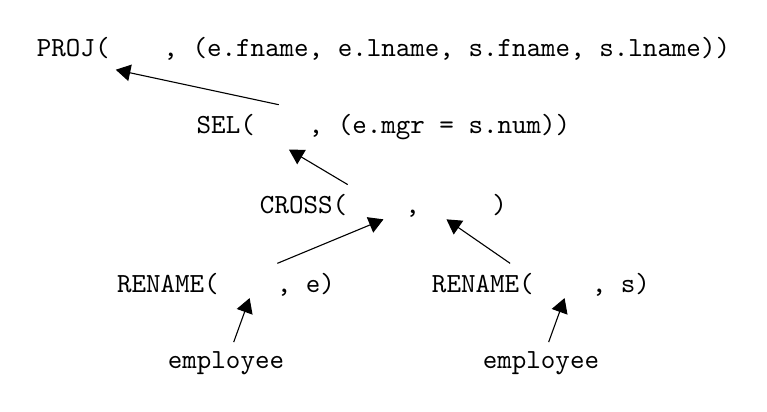
\begin{tikzpicture}
		\node (proj) at(0, 0) {\texttt{PROJ(\hspace{0.5cm} , (e.fname, e.lname, s.fname, s.lname))} };
		\node (sel) [below of =proj] {\texttt{SEL(\hspace{0.5cm} , (e.mgr = s.num))} };
		\node (cross)[below of =sel] {\texttt{CROSS(\qquad, \qquad)} };
		\node (rename1) [below of = cross, xshift=-2cm] {\texttt{RENAME(\qquad, e)}};
		\node (rename2) [below of =cross, xshift=2cm] {\texttt{RENAME(\qquad, s)}};
		\node (emp1) [below of = rename1] {\texttt{employee}};
		\node (emp2) [below of =rename2] {\texttt{employee}};

		\draw[-triangle 60] (sel) -- ($(proj.south) + (-3.4,0)$);
		\draw[-triangle 60] (cross) -- ($(sel.south) + (-1.2,0)$);
		\draw[-triangle 60] (rename1) -- ($(cross.south) + (0.0,0.1)$);
		\draw[-triangle 60] (rename2) -- ($(cross.south) + (0.8,0.1)$);
		\draw[-triangle 60] (emp1) -- ($(rename1.south) + (0.3,0.1)$);
		\draw[-triangle 60] (emp2) -- ($(rename2.south) + (0.3,0.1)$);
	\end{tikzpicture}
\paragraph{\color{solutioncolor}Anmerkung:} In der Tafelübung wird der Einfachheit halber die folgende Darstellung verwendet:
\begin{lstlisting}
- PROJ( , (e.fname, e.lname, s.fname, s.lname))
  - SEL( , (e.mgr = s.num))
    - CROSS( , )
      - RENAME( , e)
        - employee
      - RENAME( , s)
        - employee
\end{lstlisting}
	\end{solution}

\beamertxt{\pagebreak}

	\item Alle MitarbeiterInnen der Forschungsabteilung.
	\begin{lstlisting}
SELECT e.fname, e.lname, e.addr
FROM   employee e
JOIN   department d
ON     d.num = e.dep
WHERE  d.name = 'Research';
	\end{lstlisting}

	\begin{solution}
	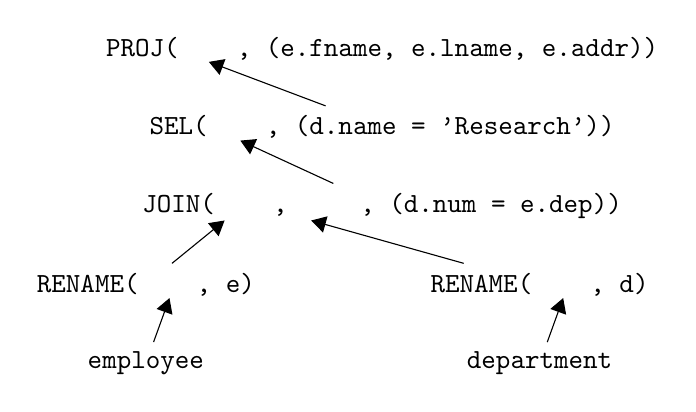
\begin{tikzpicture}
		\node (proj) at (0, 0) {\texttt{PROJ(\qquad , (e.fname, e.lname, e.addr))} };
		\node (sel)[below of =proj] {\texttt{SEL(\qquad , (d.name = 'Research'))} };

		\node (join)[below of =sel] {\texttt{JOIN(\qquad, \qquad, (d.num = e.dep))} };
		\node (renamed)[below of =join, xshift = 2cm] {\texttt{RENAME(\qquad, d)}};
		\node (renamee)[below of =join, xshift =-3cm] {\texttt{RENAME(\qquad, e)}};
		\node (dept)[below of =renamed] {\texttt{department} };
		\node (emp)[below of =renamee] {\texttt{employee} };

		\draw[-triangle 60] (dept) -- ($(renamed.south) + (0.3,0.1)$);
		\draw[-triangle 60] (emp) -- ($(renamee.south) + (0.3,0.1)$);
		\draw[-triangle 60] (renamed) -- ($(join.south) + (-0.9,0.1)$);
		\draw[-triangle 60] (renamee) -- ($(join.south) + (-2,0.1)$);
		\draw[-triangle 60] (join) -- ($(sel.south) + (-1.8,0.1)$);
		\draw[-triangle 60] (sel) -- ($(proj.south) + (-2.2,0.1)$);
	\end{tikzpicture}
	\end{solution}

  \item Alle Abteilungen mit mehr als 10 Mitarbeitern.
	\begin{lstlisting}
SELECT   d.name
FROM     employee e
JOIN     department d
ON       d.num = e.dep
GROUP BY d.num, d.name
HAVING   count(d.num) > 10
	\end{lstlisting}

	\begin{solution}
	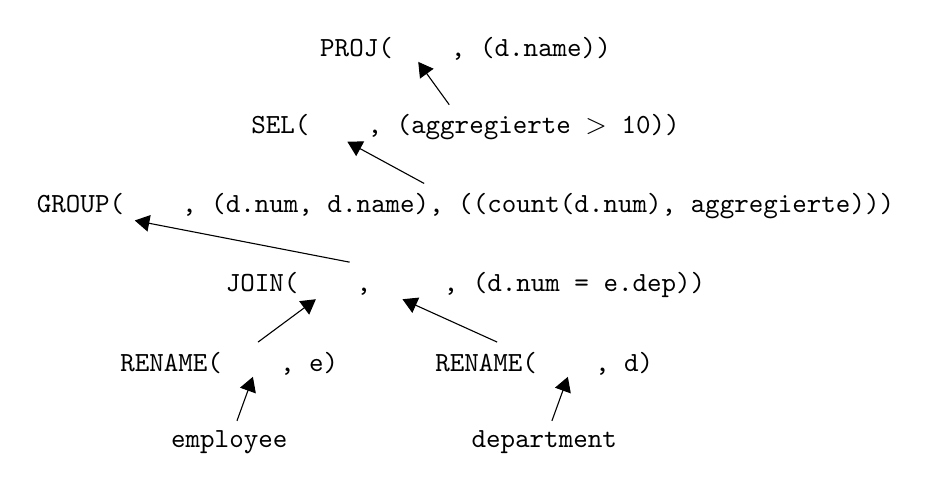
\begin{tikzpicture}
		\node (proj) at (0, 0) {\texttt{PROJ(\qquad , (d.name))} };
		\node (hav)[below of =proj] {\texttt{SEL(\qquad , (aggregierte $>$ 10))} };

		\node (group)[below of =hav] {\texttt{GROUP(\qquad , (d.num, d.name), ((count(d.num), aggregierte)))}};
		\node (join)[below of =group] {\texttt{JOIN(\qquad, \qquad, (d.num = e.dep))} };
		\node (renamed)[below of =join, xshift = 1cm] {\texttt{RENAME(\qquad, d)} };
		\node (renamee)[below of =join, xshift =-3cm] {\texttt{RENAME(\qquad, e)} };
		\node (dept)[below of =renamed] {\texttt{department} };
		\node (emp)[below of =renamee] {\texttt{employee} };

		\draw[-triangle 60] (renamed) -- ($(join.south) + (-0.8,0.1)$);
		\draw[-triangle 60] (renamee) -- ($(join.south) + (-1.9,0.1)$);
		\draw[-triangle 60] (dept) -- ($(renamed.south) + (0.3,0.1)$);
		\draw[-triangle 60] (emp) -- ($(renamee.south) + (0.3,0.1)$);
		\draw[-triangle 60] (join) -- ($(group.south) + (-4.2,0.1)$);
		\draw[-triangle 60] (group) -- ($(hav.south) + (-1.5,0.1)$);
		\draw[-triangle 60] (hav) -- ($(proj.south) + (-0.6,0.1)$);
	\end{tikzpicture}
	\end{solution}

	\item Alle MitarbeiterInnen mit Nachnamen Smith, die eine operative Abteilung leiten oder einem Projekt zugeordnet sind.
	\begin{lstlisting}
SELECT e.lname
FROM ((SELECT p.num, e.lname
    FROM   project p, department d, employee e
    WHERE  d.num = p.dep
    AND    d.mgr = e.num
  )
  UNION
  ( SELECT p.num, e.lname
    FROM   project p, works_on w, employee e
    WHERE  p.num = proj
    AND    e.num = empl
  )
)
WHERE e.lname = 'Smith';
	\end{lstlisting}

	\begin{solution}
	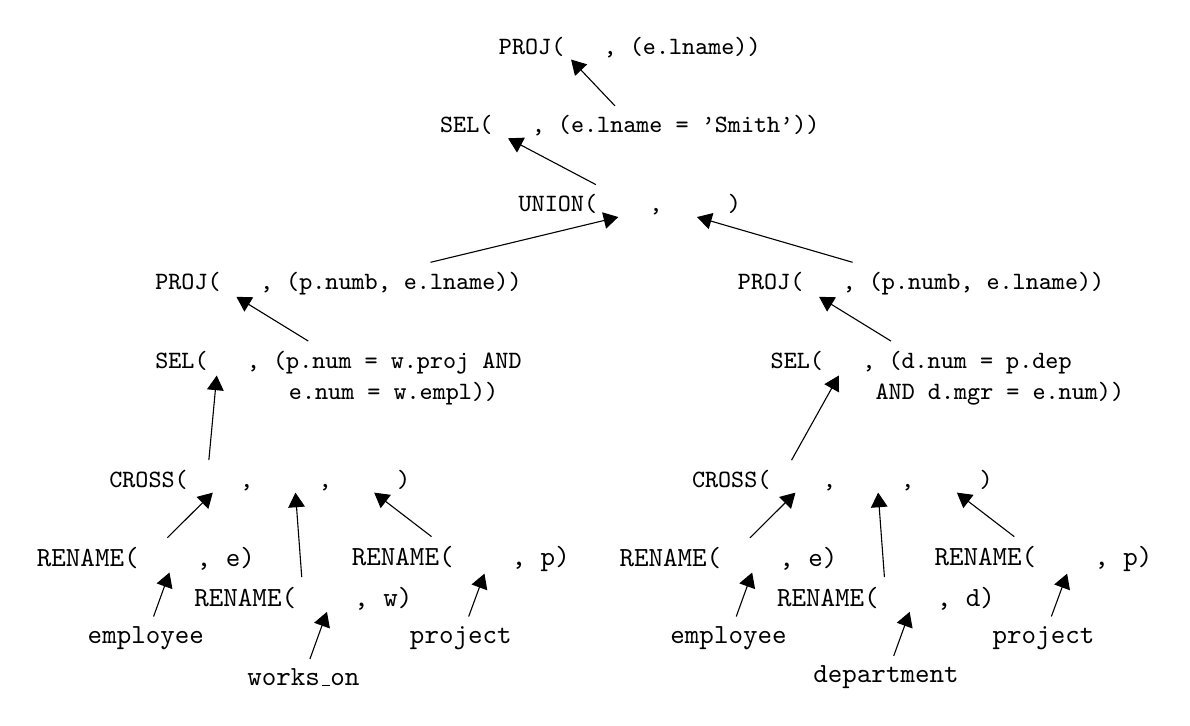
\begin{tikzpicture}
		\node (proj_top) at(0, 0) {\small{\texttt{PROJ(\hspace{0.5cm}, (e.lname))} } };
		\node (sel_top) [below of =proj_top] {\small{\texttt{SEL(\hspace{0.5cm}, (e.lname = 'Smith'))} } };
		\node (union) [below of =sel_top] {\small{\texttt{UNION(\qquad, \qquad)} } };

		\node (proj_left) [below of =union, xshift = 3.7cm] {\small{\texttt{PROJ(\hspace{0.5cm}, (p.numb, e.lname))} } };
		\node (proj_right) [below of =union, xshift = -3.7cm] {\small{\texttt{PROJ(\hspace{0.5cm}, (p.numb, e.lname))} } };

		\node (sel_left) [below of =proj_left] {\small{\texttt{SEL(\hspace{0.5cm}, (d.num = p.dep} } };
		\node (sel_left2) [below of =sel_left, xshift =1cm, yshift = 0.6cm] {\small{\texttt{AND d.mgr = e.num))} } };
		\node (sel_right) [below of =proj_right, xshift =0cm] {\small{\texttt{SEL(\hspace{0.5cm}, (p.num = w.proj AND} } };
		\node (sel_right2) [below of =sel_right, xshift =0.7cm, yshift = 0.6cm] {\small{\texttt{e.num = w.empl))} } };

		\node (cross_left) [below of =sel_left, xshift =-1cm, yshift =-0.5cm] {\small{\texttt{CROSS(\qquad, \qquad, \qquad)} } };
		\node (cross_right) [below of =sel_right, xshift =-1cm, yshift =-0.5cm] {\small{\texttt{CROSS(\qquad, \qquad, \qquad)} } };

		\node (rename_emp_left) [below of =cross_left, xshift =-1.5cm] {\texttt{RENAME(\qquad, e)}};
		\node (rename_dept_left) [below of =cross_left, xshift =0.5cm, yshift =-0.5cm] {\texttt{RENAME(\qquad, d)} };
		\node (rename_project_left) [below of =cross_left, xshift =2.5cm] {\texttt{RENAME(\qquad, p)}};
		\node (rename_emp_right) [below of =cross_right, xshift =-1.5cm] {\texttt{RENAME(\qquad, e)}};
		\node (rename_works_right) [below of =cross_right, xshift =0.5cm, yshift =-0.5cm] {\texttt{RENAME(\qquad, w)}};
		\node (rename_project_right) [below of =cross_right, xshift =2.5cm] {\texttt{RENAME(\qquad, p)}};

		\node (emp_left) [below of =rename_emp_left] {\texttt{employee} };
		\node (dept_left) [below of =rename_dept_left] {\texttt{department}};
		\node (project_left) [below of =rename_project_left] {\texttt{project} };
		\node (emp_right) [below of =rename_emp_right] {\texttt{employee} };
		\node (works_right) [below of =rename_works_right] {\texttt{works\_on} };
		\node (project_right) [below of =rename_project_right] {\texttt{project} };

		\draw[-triangle 60] (sel_top) -- ($(proj_top.south) + (-0.8,0.1)$);
		\draw[-triangle 60] (union) -- ($(sel_top.south) + (-1.6,0.1)$);

		\draw[-triangle 60] (proj_left) -- ($(union.south) + (0.8, 0.1)$);
		\draw[-triangle 60] (proj_right) -- ($(union.south) + (-0.2, 0.1)$);

		\draw[-triangle 60] (sel_left) -- ($(proj_left.south) + (-1.35,0.1)$);
		\draw[-triangle 60] (sel_right) -- ($(proj_right.south) + (-1.35,0.1)$);

		\draw[-triangle 60] ($(cross_left.north) + (-0.7, 0 )$) -- ($(sel_left.south) + (-1.1,0.1)$);
		\draw[-triangle 60] ($(cross_right.north) + (-0.7, 0 )$) -- ($(sel_right.south) + (-1.6,0.1)$);

		\draw[-triangle 60] (rename_emp_left) -- ($(cross_left.south) + (-0.65,0.1)$);
		\draw[-triangle 60] (rename_dept_left) -- ($(cross_left.south) + (0.4,0.1)$);
		\draw[-triangle 60] (rename_project_left) -- ($(cross_left.south) + (1.4,0.1)$);
		\draw[-triangle 60] (rename_emp_right) -- ($(cross_right.south) + (-0.65,0.1)$);
		\draw[-triangle 60] (rename_works_right) -- ($(cross_right.south) + (0.4,0.1)$);
		\draw[-triangle 60] (rename_project_right) -- ($(cross_right.south) + (1.4,0.1)$);

		\draw[-triangle 60] (emp_left) -- ($(rename_emp_left.south) + (0.3,0.1)$);
		\draw[-triangle 60] (dept_left) -- ($(rename_dept_left.south) + (0.3,0.1)$);
		\draw[-triangle 60] (project_left) -- ($(rename_project_left.south) + (0.3,0.1)$);
		\draw[-triangle 60] (emp_right) -- ($(rename_emp_right.south) + (0.3,0.1)$);
		\draw[-triangle 60] (works_right) -- ($(rename_works_right.south) + (0.3,0.1)$);
		\draw[-triangle 60] (project_right) -- ($(rename_project_right.south) + (0.3,0.1)$);
	\end{tikzpicture}
	\end{solution}

\end{enumerate}


\beamertxt{\pagebreak}
\section{Unnesting}
\label{unnesting}

Gegeben seien folgende Relationen eines Datenbankschemas:

\texttt{Studierende (\underline{matrikelnr}, name)} \\
\texttt{Noten (\underline{pruefungsnr, matrikelnr}, note, semester, datum)}

Eine Anfrage, die für jede(n) Studierende(n) die beste Prüfungsleistung ermittelt,
könnte wie folgt aussehen:

\cprotEnv
\begin{normalText}
\begin{lstlisting}
SELECT s.name, n.pruefungsnr, n.note
FROM   Studierende s, Noten n
WHERE  s.matrikelnr = n.matrikelnr AND
       n.note = (SELECT min(n2.note)
                 FROM Noten n2
                 WHERE s.matrikelnr = n2.matrikelnr);
\end{lstlisting}
\end{normalText}

\cprotEnv
\begin{beamerText}
\begin{lstlisting}
SELECT s.name, n.pruefungsnr, n.note
FROM   Studierende s, Noten n
WHERE  s.matrikelnr = n.matrikelnr AND
    n.note = (SELECT min(n2.note)
              FROM Noten n2
              WHERE s.matrikelnr = n2.matrikelnr);
\end{lstlisting}
\end{beamerText}


\begin{note}
Für jede eingetragene Note wird geprüft,
ob es die jeweils beste der/des aktuellen Studierenden ist.
\end{note}

\begin{enumerate}[a)]

  \item \label{a} Bewerten Sie die Anfrage im Hinblick auf das zu erwartende Leistungsverhalten
    und die Optimierungsmöglichkeiten.

\begin{solution}
Aus Sicht des Leistungsverhaltens ist diese Anfrage problematisch,
weil die Unteranfrage für jedes einzelne Studierende-Noten-Paar
komplett wiederholt werden muss.
\end{solution}

  \item Schreiben Sie die Anfrage so um, dass es die unter \ref{a}) genannten
    Probleme löst und die Bearbeitung optimiert werden kann.

\cprotEnv
\begin{solution}
Das Problem ist, wie bereits oben genannt, die Abhängigkeit der Unteranfrage
von \texttt{s.matrikelnr} der oberen Anfrage.
Es handelt sich also, wie im ersten Übungsblatt bereits kennengelernt,
um eine \emph{korrelierte Unteranfrage}.

Ziel ist es also, die Anfrage so umzuschreiben,
dass die Abhängigkeit eliminiert wird.
Das ist in diesem Fall relativ einfach.
Die Grundidee besteht darin, die beste Note jedes Studierenden bereits
in der Notentabelle zu ermitteln und das Ergebnis mithilfe eines Kreuzprodukts
mit der Studierenden-Relation zu verbinden:

\begin{lstlisting}
SELECT s.name, n.pruefungsnr, n.note
FROM   Studierende s, Noten n,
       (SELECT  n2.matrikelnr as matrikelnr,
                min(n2.note) as beste
        FROM    Noten n2
        GROUP BY n2.matrikelnr) m
WHERE  s.matrikelnr = n.matrikelnr AND
       s.matrikelnr = m.matrikelnr AND
       n.note = m.beste;
\end{lstlisting}

\cprotEnv
\begin{note}
Die ganze Anfrage lässt sich auch alternativ komplett ohne Unteranfrage schreiben:

\begin{lstlisting}
SELECT   s.name, n.pruefungsnr, n.note
FROM     Studierende s, Noten n, Noten n2
WHERE    n.matrikelnr = n2.matrikelnr
AND      s.matrikelnr = n.matrikelnr
GROUP BY n.matrikelnr, s.name, n.pruefungsnr, n.note
HAVING   n.note = min(n2.note)
\end{lstlisting}
\end{note}

Nun muss die Unteranfrage nur noch einmal evaluiert werden.
Das Ergebnis kann mittels bereits kennengelernter JOIN-Mechanismen dann
mit den beiden Relationen \texttt{Studierende} und \texttt{Noten} verknüpft werden.

Diese Optimierung kann so vom DBMS automatisch durchgeführt werden.
Sie ist vergleichsweise leicht erkennbar und wie man sieht, wurde die Unteranfrage
nur in die FROM-Klausel verschoben und durch ein Symbol (\texttt{m.beste}) ersetzt.

Wird eine korrelierte Unteranfrage auf diese Art aufgelöst,
spricht man von \emph{Unnesting}.
\end{solution}

\end{enumerate}


\beamertxt{\pagebreak}
\begin{deeper}
\section{Unnesting 2}
\label{unnesting2}

Gegeben seien folgende Relationen eines Datenbankschemas, die aus Aufgabe \ref{unnesting} bekannt sind:

\texttt{Studierende (\underline{matrikelnr}, name)} \\
\texttt{Noten (\underline{pruefungsnr, matrikelnr}, note, semester, datum)}

Bauen Sie die folgenden SQL-Anfragen so um, dass keine korrelierten Unteranfragen mehr vorliegen.

\cprotEnv
\begin{normalText}
Hinweis: Es ist sinnvoll, die Teilaufgaben in der gegebenen Reihenfolge zu bearbeiten, da jede Teilaufgabe eine neue Problemstellung zur vorhergehenden Teilaufgabe hinzufügt.

\begin{enumerate}[a)]

\item

\begin{lstlisting}
-- Die Matrikelnummern der besten Studierenden jedes Pruefungstags
SELECT n.matrikelnr, n.datum
FROM   Noten n
WHERE  n.note = (SELECT min (n2.note)
                 FROM   Noten n2
                 WHERE  n.datum = n2.datum);
\end{lstlisting} \label{first}

\cprotEnv
\begin{note}
\begin{lstlisting}
SELECT n.matrikelnr, n.datum
FROM   Noten n,
(
 SELECT   min(n2.note) as min, n2.datum
 FROM     Noten n2
 GROUP BY n2.datum
) m
WHERE n.note = m.min AND n.datum = m.datum
\end{lstlisting}
\end{note}

\item

\begin{lstlisting}
-- Zu jeder Pruefungsteilnahme die bis zu dem Datum
-- besten Noten des Pruefungsteilnehmers
SELECT n.matrikelnr, n.datum, n2.note, n2.pruefungsnr
FROM   Noten n, Noten n2
WHERE  n.matrikelnr = n2.matrikelnr
AND    n2.datum < n.datum
AND    n2.note = (SELECT min(n3.note)
                  FROM   Noten n3
                  WHERE  n3.datum < n.datum
		  AND    n3.matrikelnr = n.matrikelnr)
\end{lstlisting}

\cprotEnv
\begin{note}
\begin{lstlisting}
SELECT   n.matrikelnr, n.datum, n2.note, n2.pruefungsnr
FROM     Noten n, Noten n2, Noten n3
WHERE    n2.matrikelnr = n.matrikelnr
AND      n3.matrikelnr = n.matrikelnr
AND      n2.datum  < n.datum
AND      n3.datum < n.datum
GROUP BY n.matrikelnr, n.datum, n2.note, n2.pruefungsr
HAVING   n2.note = min(n3.note)
\end{lstlisting}

Alternativ, näher an der ML:

\begin{lstlisting}
SELECT   n.matrikelnr, n.datum, n2.note, n2.pruefungsnr
FROM     Noten n, Noten n2,
(
 SELECT   min(n3.note) as min, n3.datum, n3.matrikelnr
 FROM     Noten n3
 GROUP BY n3.datum, n3.matrikelnr
) m
WHERE    n.matrikelnr = n2.matrikelnr
AND      m.matrikelnr = n.matrikelnr
AND      m.datum  < n.datum
AND      n2.datum < n.datum
GROUP BY n.matrikelnr, n.datum, n2.note, n2.pruefungsr
HAVING   n2.note = min(m.min)
\end{lstlisting}
\end{note}

\item

\begin{lstlisting}
-- Fuer eine lustige Lotterie werden zu jeder Pruefung
-- die Studierenden gesucht, deren Anzahl an
-- Pruefungsteilnahmen vor dem Tag der Pruefung der
-- Pruefungsnummer entspricht
SELECT n.pruefungsnr, n.matrikelnr
FROM Noten n
WHERE n.pruefungsnr = (SELECT count(*)
                       FROM   Noten n2
                       WHERE  n2.matrikelnr = n.matrikelnr
                       AND    n2.datum < n.datum)
\end{lstlisting}

\cprotEnv
\begin{note}
\begin{lstlisting}
SELECT   n.matrikelnr, n.pruefungsnr
FROM     Noten n, Noten n2
WHERE    n2.matrikelnr = n.matrikelnr
AND      n2.datum < n.datum
GROUP BY n.matrikelnr, n.pruefungsnr
HAVING   n.pruefungsnr = count(*)
\end{lstlisting}

Alternativ, näher an der ML:

\begin{lstlisting}
SELECT   n.matrikelnr, n.pruefungsnr
FROM     Noten n,
(
SELECT   count(n2.note) as count, n2.matrikelnr, n2.datum
FROM     Noten n2
GROUP BY n2.datum, n2.matrikelnr
) m
WHERE    n.matrikelnr = m.matrikelnr
AND      m.datum < n.datum
GROUP BY n.matrikelnr, n.pruefungsnr
HAVING   n.pruefungsnr = sum(m.count)
\end{lstlisting}
\end{note}

\end{enumerate}
\end{normalText}

\end{deeper}

\beamertxt{\pagebreak}
\section{Optimierung im Betrieb -- Beispiele}

Große Datenbanksysteme wie beispielsweise Oracle bieten Administratoren die Möglichkeit,
im Betrieb Einfluss auf bestimmte Optimierungsparameter zu nehmen.
Welche Informationen benötigt der Administrator und wie könnten Schnittstellen für diese Einflussnahme aussehen?

\begin{note}
Diskussionsaufgabe! Im folgenden ist beispielhaft beschrieben,
welche Möglichkeiten Oracle unter anderem bietet.

Darüber hinaus sind viele weitere denkbar und auch implementiert.
\end{note}

\cprotEnv
\begin{solution}
Wie Sie in den letzten Blättern kennengelernt haben,
nutzen Datenbanksysteme häufig bereits verschiedenste Algorithmen,
um das Leistungsverhalten zu steigern.
Dazu müssen verschiedene Hilfsstrukturen mitgeführt werden.

Der Administrator als Mensch hat unter Umständen durch Kenntnis
des gesamten Systems (also Hardware, Betriebssystem, Anwendung etc.)
die Möglichkeit, bessere Aussagen zu möglichen Optimierungen zu treffen,
als es das Datenbankverwaltungssystem durch reines Mitführen von Statistiken kann.

Damit der Administrator die vom System getroffenen Entscheidungen
jedoch bewerten kann, benötigt er Zugriff auf die internen Statistiken,
auf Basis derer das Datenbankverwaltungssystem die Entscheidungen trifft.

    Bei Oracle ist es nicht nur möglich,
    die internen Statistiken über die Datenbank selbst zu betrachten.
    Es werden darüber hinaus auch Statistiken
    über die ausgeführten SQL-Anfragen gesammelt,
    wie z.\,B. Ausführungszeiten, generierte Ausführungspläne
    etc.\footnote{\url{http://docs.oracle.com/cd/B19306_01/server.102/b14211/sql_1016.htm\#i26072}}

    Stellt der Administrator nun fest, dass für eine bestimmte Anfrage
    regelmäßig ein (in der Praxis) schlechter Ausführungsplan gewählt wird,
    kann er z.B. mit sogenannten \emph{HINTS} die Ausführung beeinflussen.
    Dabei wird in die SQL-Anfrage selbst ein Kommentar geschrieben,
    der vom Optimierer interpretiert
    wird.\footnote{\url{http://docs.oracle.com/cd/B19306_01/server.102/b14211/hintsref.htm}}

    Ein solcher HINT könnte z.\,B. so aussehen:

\begin{lstlisting}
    SELECT /*+ USE_NL(e d) */ e.fname, e.lname, e.addr
        FROM employee e
        JOIN department d
        ON d.num = e.dep
        WHERE d.name = 'Research';
\end{lstlisting}

    Damit wird dem Optimierer empfohlen, einen Nested-Loop-Join zu verwenden.
    Zu beachten ist jedoch, dass es sich dabei
    -- wie der Begriff \emph{HINT} schon andeutet --
    nicht um eine Anweisung handelt,
    sondern wie gesagt vielmehr um eine \textbf{Empfehlung}.
    Der Optimierer kann sich trotzdem darüber hinwegsetzen.
    Der Administrator erkennt dies dann wieder in den Statistiken.


    Das ständige (oder regelmäßige) Mitführen von Statistiken generiert
    auf dem System allerdings zusätzliche Last,
    entweder durch ständiges Aktualisieren von Statistikdaten
    oder durch regelmäßige Aktualisierungsläufe.

    Oracle bietet daher einen weiteren ganz grundsätzlichen Ansatz an.
    Es ist möglich, den kostenbasierten Optimierer zu deaktivieren
    und Ausführungspläne z.\,B. nach festen Regeln erstellen zu
    lassen.\footnote{\url{http://docs.oracle.com/cd/B19306_01/server.102/b14211/optimops.htm}}
    Das bietet den Vorteil, dass auf das Mitführen von Statistiken
    (vor allem wie viele Tupel in einer Relation sind, Selektivitäten etc.)
    weitgehend verzichtet werden kann.
    Ist also absehbar,
    dass der mit den Statistiken verbundene Aufwand größer ist
    als der Nutzen der kostenbasierten Wahl der Ausführungspläne,
    kann auch
    auf den kostenbasierten Optimierer komplett verzichtet werden.

    Weitere mögliche Ideen, unabhängig vom verwendeten System:
    \begin{itemize}
        \item Wenn häufig eine komplizierte JOIN-Abfrage durchgeführt wird:
            \textbf{Materialisierte Sicht} anlegen
            (und die Anfragen daran anpassen oder dem Optimierer beibringen,
            dass er die Sicht automatisch nutzen kann)
        \item Wenn in der Selektion häufig ein Ausdruck verwendet wird,
            der die Nutzung eines bisher verfügbaren Index unmöglich macht:
            \textbf{Function-Based Index} über diesen Ausdruck anlegen
        \item Puffer vergrößern
        \item schnellere / besser geeignete Hintergrundspeicher
    \end{itemize}
\end{solution}


\beamertxt{\pagebreak}
\begin{deeper}
\section{Schichtenmodell}

Ordnen Sie die folgenden Begriffe, Funktionen, Beschreibungen und Schnittstellen in das Schichtenmodell eines Datenbanksystems ein, indem Sie sie an der richtigen Stelle in die auf der nächsten Seite dargestellte Grafik eintragen.

\cprotEnv
\begin{normalText}
\begin{minipage}[t]{0.49\textwidth}
\begin{itemize}\setlength\itemsep{0em}
    \item Abbildung eines Dateinamens auf Folge von Blöcken
    \item Anfrage verarbeiten
    \item Anwendungsstrukturen
    \item append(Datei, Blockanzahl)
    \item Ausführungsplanerstellung
    \item B*-Baum
    \item Blockdatei
    \item blockorientierte Dateischnittstelle
    \item Felder/Attribute
    \item fix(Segment, Seite)
    \item Geräteschnittstelle
    \item Interne Satzschnittstelle
    \item Kanalkommandos
    \item Mengenorientierte DB-Schnittstelle
\end{itemize}
\end{minipage}
\begin{minipage}[t]{0.49\textwidth}
\begin{itemize}\setlength\itemsep{0em}
    \item Overflow-Buckets
    \item prepareStatement(sql)
    \item Projektion (C-Store)
    \item R-Baum
    \item readBlock(LBA-Nummer)
    \item read(TID)
    \item Schattenspeicher
    \item Schema
    \item Seitenorientierte Pufferschnittstelle
    \item Seitentabelle
    \item sequenzielle Satzdatei
    \item SQL-String parsen
    \item TID
    \item Tupelzeiger
    \item unfix(Segment, Seite)
\end{itemize}
\end{minipage}


\begin{center}
\ifnotes
	\includegraphics[width=0.9\textwidth]{Pictures/UeIDB11_Optimierung_Schichtenmodell_ML.pdf}
\else
	\includegraphics[width=0.9\textwidth]{Pictures/UeIDB11_Optimierung_Schichtenmodell.pdf}
\fi
\end{center}
\end{normalText}

\end{deeper}

\end{document}
